\section{Spintronics Concepts}

\subsection{Antiferromagnets}

An antiferromagnet is a magnetic material in which neighboring magnetic moments
prefer an antiparallel arrangement.  The opposing moments can compensate,
giving little or no net magnetization even though the material has long-range
magnetic order.  Its order is therefore described more naturally by a N\'eel
vector than by the net magnetization alone~\cite{xu2023field-free-afm}.

\subsubsection{A-Type Antiferromagnet}

An A-type antiferromagnet consists of ferromagnetic planes stacked
antiferromagnetically: spins within each plane point in the same direction,
all spins in the next plane point in the opposite direction, and the pattern
repeats along the stacking direction.  The word \emph{plane} refers to the
crystallographic planes selected by the exchange interactions in a particular
material.  Figure~\ref{fig:a-type-afm-stacking} chooses the $z$ axis as the
stacking direction as an illustrative convention, not as a universal crystal
orientation.

\paragraph{Source status.}
\textbf{Reference needed.}  This A-type structural classification was supplied
directly for these notes and still needs a dedicated literature reference.

\begin{figure}[htbp]
    \centering
    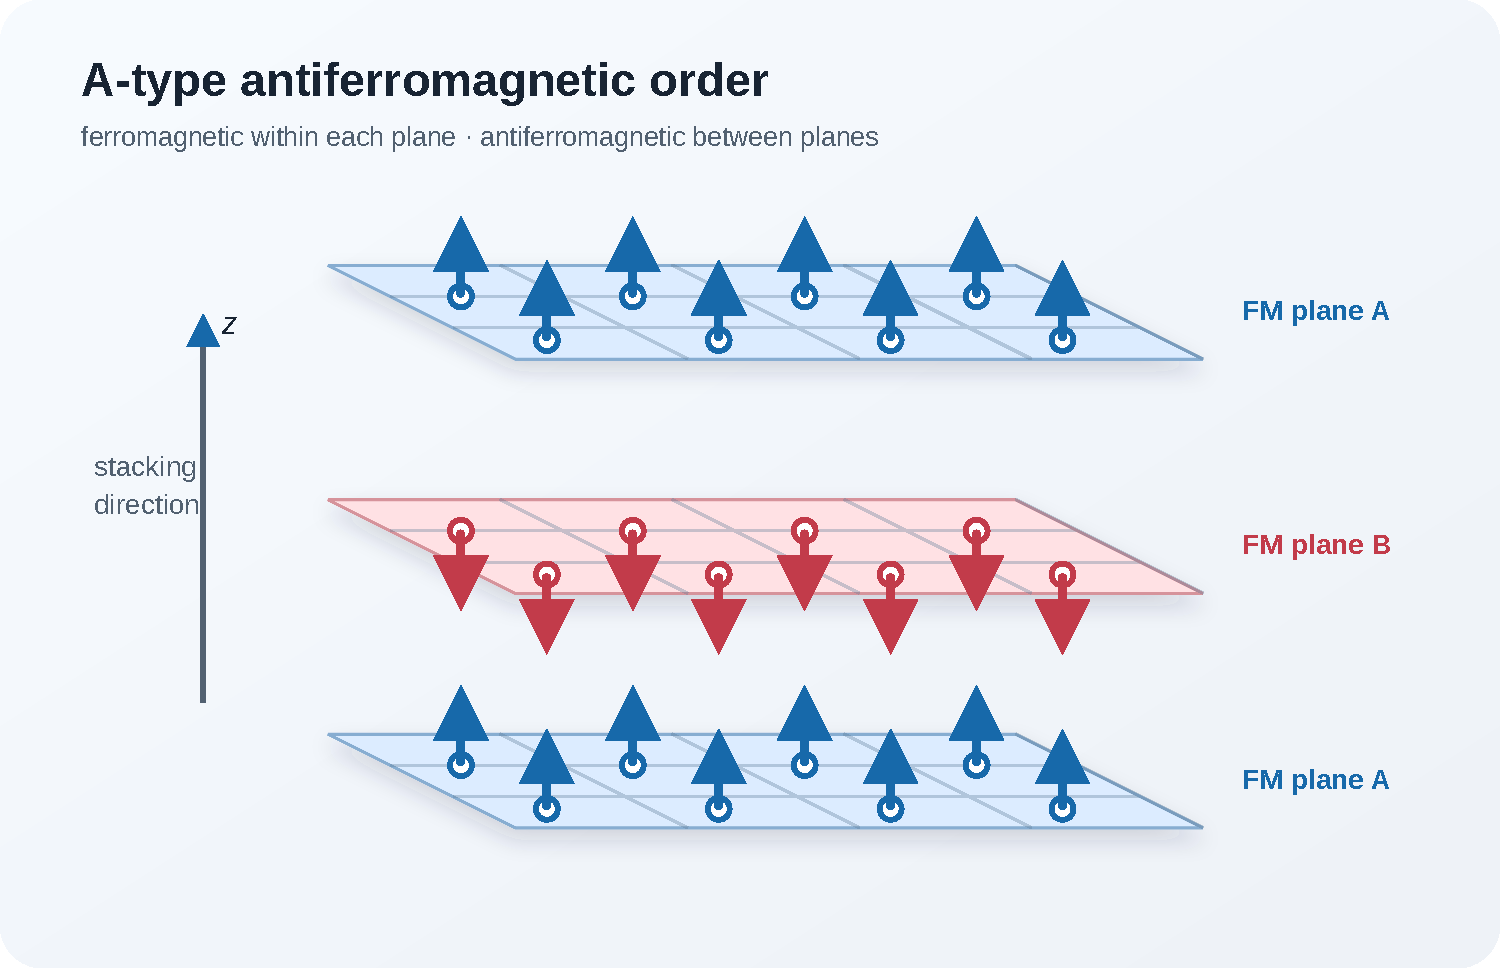
\includegraphics[width=0.92\linewidth]{images/a-type-afm-stacking.pdf}
    \caption{A-type antiferromagnetic stacking: ferromagnetic planes alternate
        in direction.  Original schematic; the physical classification follows
        the provisional description above and therefore shares its
        \textbf{reference-needed} status.}
    \label{fig:a-type-afm-stacking}
\end{figure}

For classical unit spins $\svec_i$, the exchange part of the atomistic
Hamiltonian can be written in the ASTRO sign convention as~\cite{astro-code}
\begin{equation}
    \mathcal{H}_{\mathrm{ex}}
    = \frac{1}{2}\sum_{i\ne j}J_{ij}\,\svec_i\cdot\svec_j.
    \label{eq:a-type-exchange}
\end{equation}
In this convention, A-type order is favored by
\begin{equation}
    J_{\parallel}<0,
    \qquad
    J_{\perp}>0,
    \label{eq:a-type-exchange-signs}
\end{equation}
where $J_{\parallel}$ couples neighbors within a plane and $J_{\perp}$ couples
neighbors in adjacent planes.  Thus the in-plane bonds favor parallel
alignment, whereas the interplane bonds favor antiparallel alignment.  Some
publications place a minus sign in front of the exchange sum; their signs of
$J$ are reversed.  The sign convention and pair counting in
Eq.~\eqref{eq:a-type-exchange} are the same as those used in the full atomistic
Hamiltonian in Eq.~\eqref{eq:atomistic-hamiltonian} and in ASTRO~\cite{astro-code}.

\begin{figure}[htbp]
    \centering
    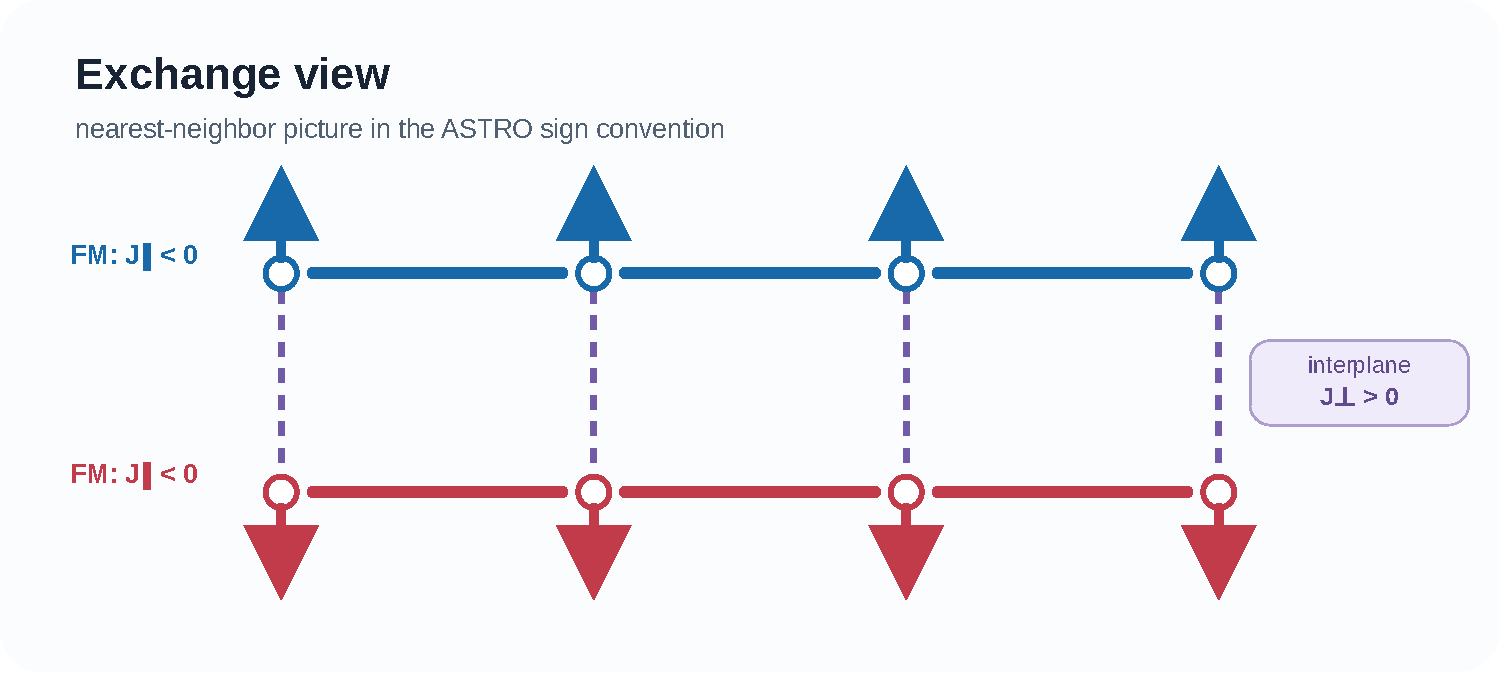
\includegraphics[width=0.95\linewidth]{images/a-type-afm-exchange.pdf}
    \caption{Exchange pattern for A-type order: parallel bonds within a layer
        and antiparallel bonds between layers.  Original schematic based on the
        cited ASTRO exchange-sign convention~\cite{astro-code}; the A-type
        classification itself remains \textbf{reference needed}.}
    \label{fig:a-type-afm-exchange}
\end{figure}

For two equivalent alternating layers with normalized layer magnetizations
$\mathbf{m}_A$ and $\mathbf{m}_B$, define the net and N\'eel order parameters
as~\cite{xu2023field-free-afm}
\begin{equation}
    \mathbf{m}=\frac{\mathbf{m}_A+\mathbf{m}_B}{2},
    \qquad
    \mathbf{n}=\frac{\mathbf{m}_A-\mathbf{m}_B}{2}.
    \label{eq:a-type-order-parameters}
\end{equation}
For an ideal compensated A-type state, these definitions give
\begin{equation}
    \mathbf{m}_B=-\mathbf{m}_A,
    \qquad
    \mathbf{m}=\mathbf{0},
    \qquad
    \lvert\mathbf{n}\rvert=1.
    \label{eq:a-type-compensated-state}
\end{equation}

The defining feature is therefore not simply zero magnetization.  It is the
specific spatial pattern of ferromagnetic order in two directions and
antiferromagnetic alternation in the third.  This distinguishes A-type order
from G-type antiferromagnetism, in which every nearest neighbor is
antiparallel, and C-type order, in which ferromagnetic chains are coupled
antiferromagnetically.  \textbf{Reference needed} for this final classification
comparison.
